\documentclass[11pt,legalpaper]{article}
\usepackage[utf8]{inputenc}
\usepackage[english]{babel}
\usepackage{bilal2vec}

\begin{document}

SE 390 — Project Task 2

Bilal Khan (b54khan@uwaterloo.ca) and Bohdan Hrotovytskyy (bhrotovy@uwaterloo.ca)

To run the code properly and plot all the figures copy the code into a jupyter notebook and run each plot cell individually.

\textbf{Item 1:} Our inputs are defined over a time period of $15$ seconds where one timestep lasts $0.001$s. In numpy, we can represent this as a two-dimensional vector of length $15,000$. We can generate the two output signals $y_{11}, y_{12}, y_{21}, y_{22}$ by passing the inputs through the simulator \mintinline{python}{y = sm.sim(u)} and then accessing the i-th component of the output system.

\textbf{Item 2:} We design a third-order low pass filter in the form $G(s) = 1 / ((1 + \tau s)^3)$. We choose $\omega_c = 100, \tau = 1 / \omega_c$ using guess-and-check to find a good value for $\omega_c$ so that the resulting filtered outputs are close to the original outputs.

\textbf{Item 3:} The other signals that we need for the algorithm (as explained in class and the paper) are the first derivatives of the inputs and the first and second derivatives of our filtered outputs. Note that we compute these signals from the denoised filtered signals we found in item 2. We numerically compute them using finite differences in numpy with \mintinline{python}{np.diff(signal)/dt}.

\textbf{Item 4:} We plot the signals below:

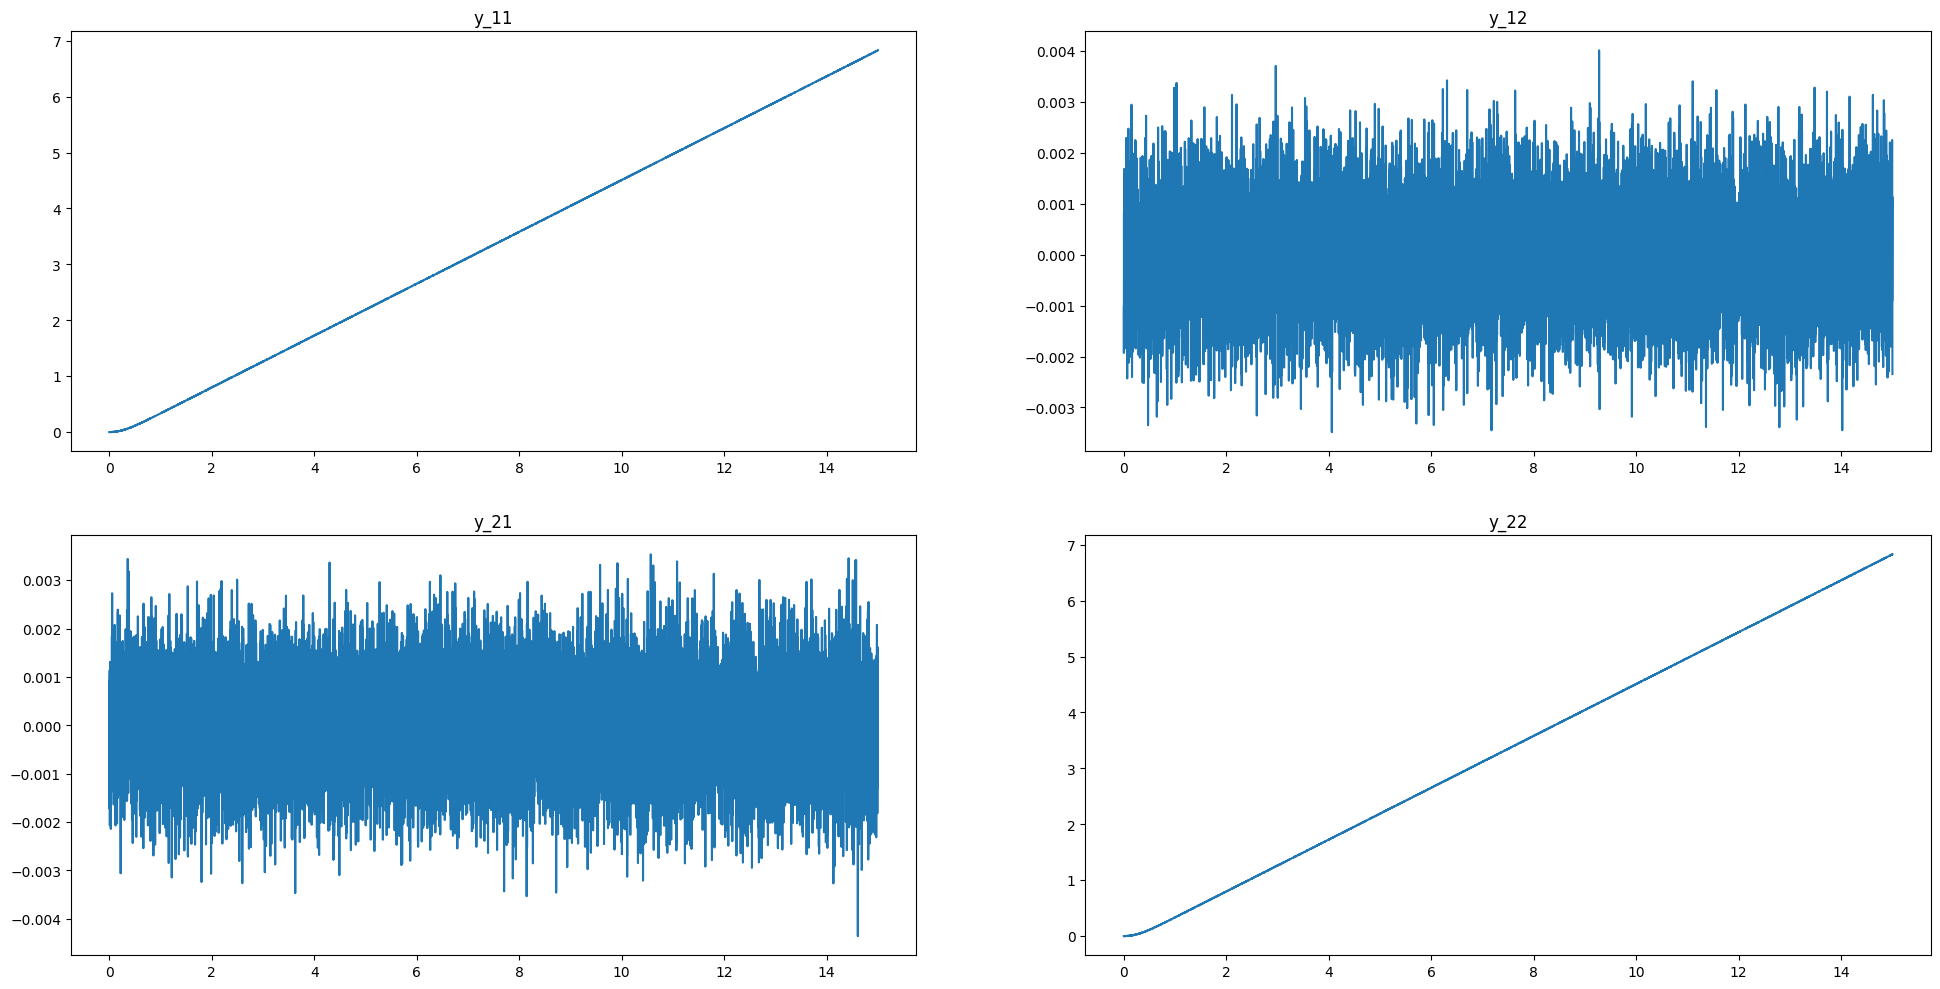
\includegraphics[width=450pt]{p2_1.png}

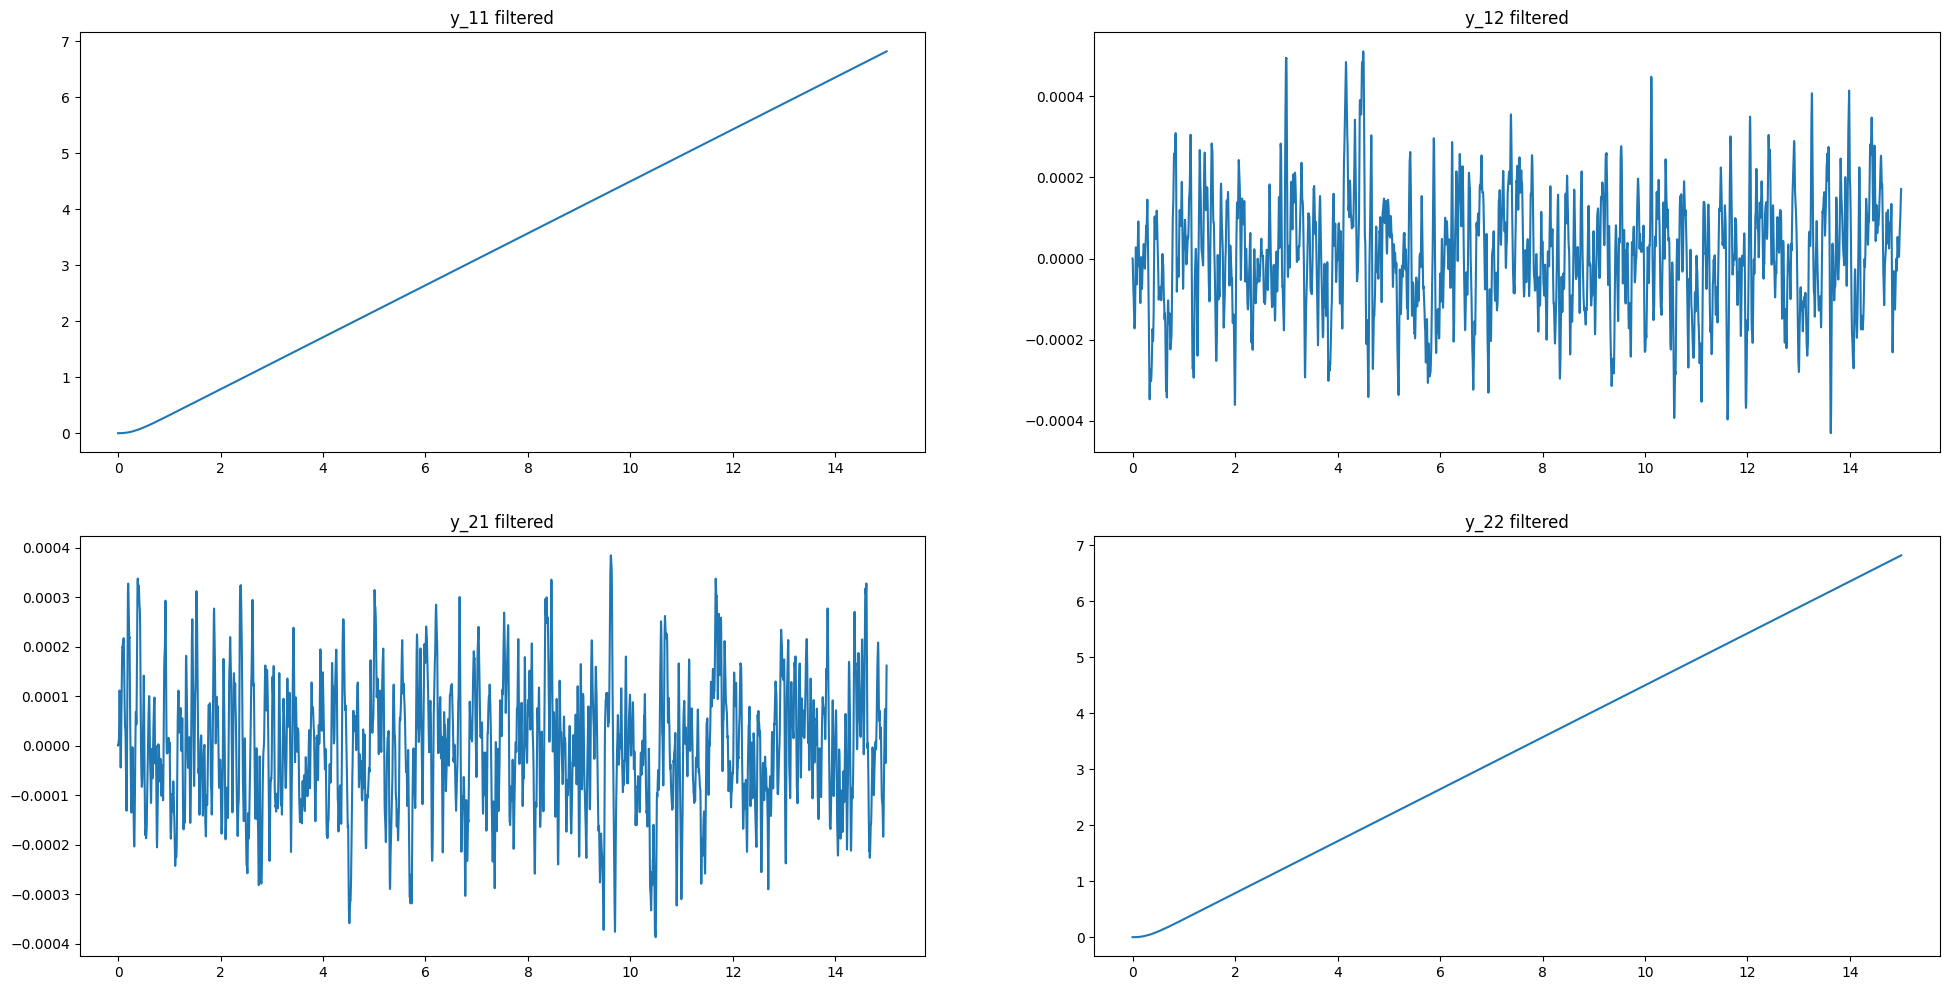
\includegraphics[width=450pt]{p2_2.png}

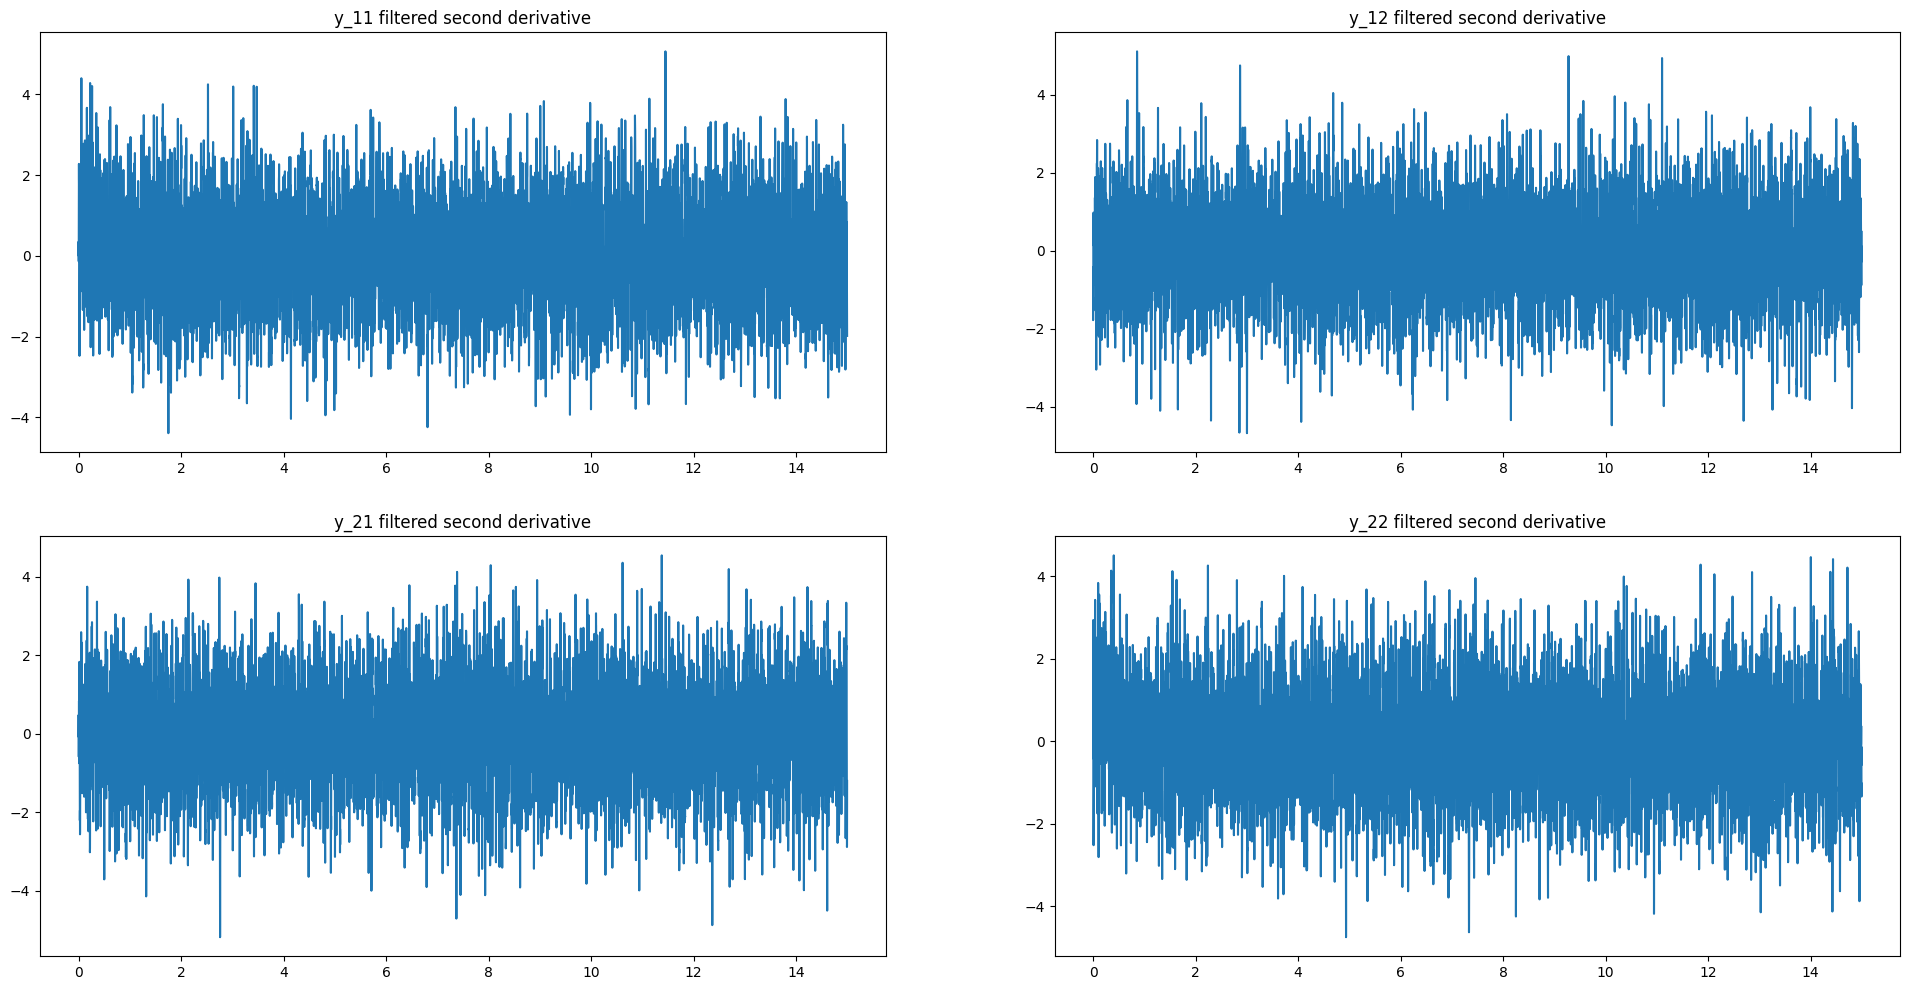
\includegraphics[width=450pt]{p2_3.png}

\textbf{Item 5:}

Refer to the code block marked "TASK 5" for full details but we use \mintinline{python}{np.linalg.lstsq} (as stated in class) to find the coefficients of the transfer function by performing least squares on each transfer function's corresponding differential equation. Our transfer functions are then: $G_{11}(s) = \frac{-8.715*10^{-15} s + 1.287}{s^2 + 2.736 s + 0.004176}$, $G_{12}(s) = \frac{0s + 0}{0s^2 + 0s + 1}$, $G_{21}(s) = \frac{1.208*10^{-13}s}{s^2 + 15.43 s + 3464}$, $G_{22}(s) = \frac{ -4.829*10^{-15}s + 1.29}{s^2 + 2.743 s + 0.003792}$

\textbf{Item 6:} The yellow line is our identified transfer function and the blue line is the original transfer function. We can see that the identified transfer function is very close to the original transfer function for $y_{11}$ and $y_{22}$. Since $y_{12}$ and $y_{21}$ are random noise signals that are very close to zero, our identified second-order transfer functions approximate them as such.

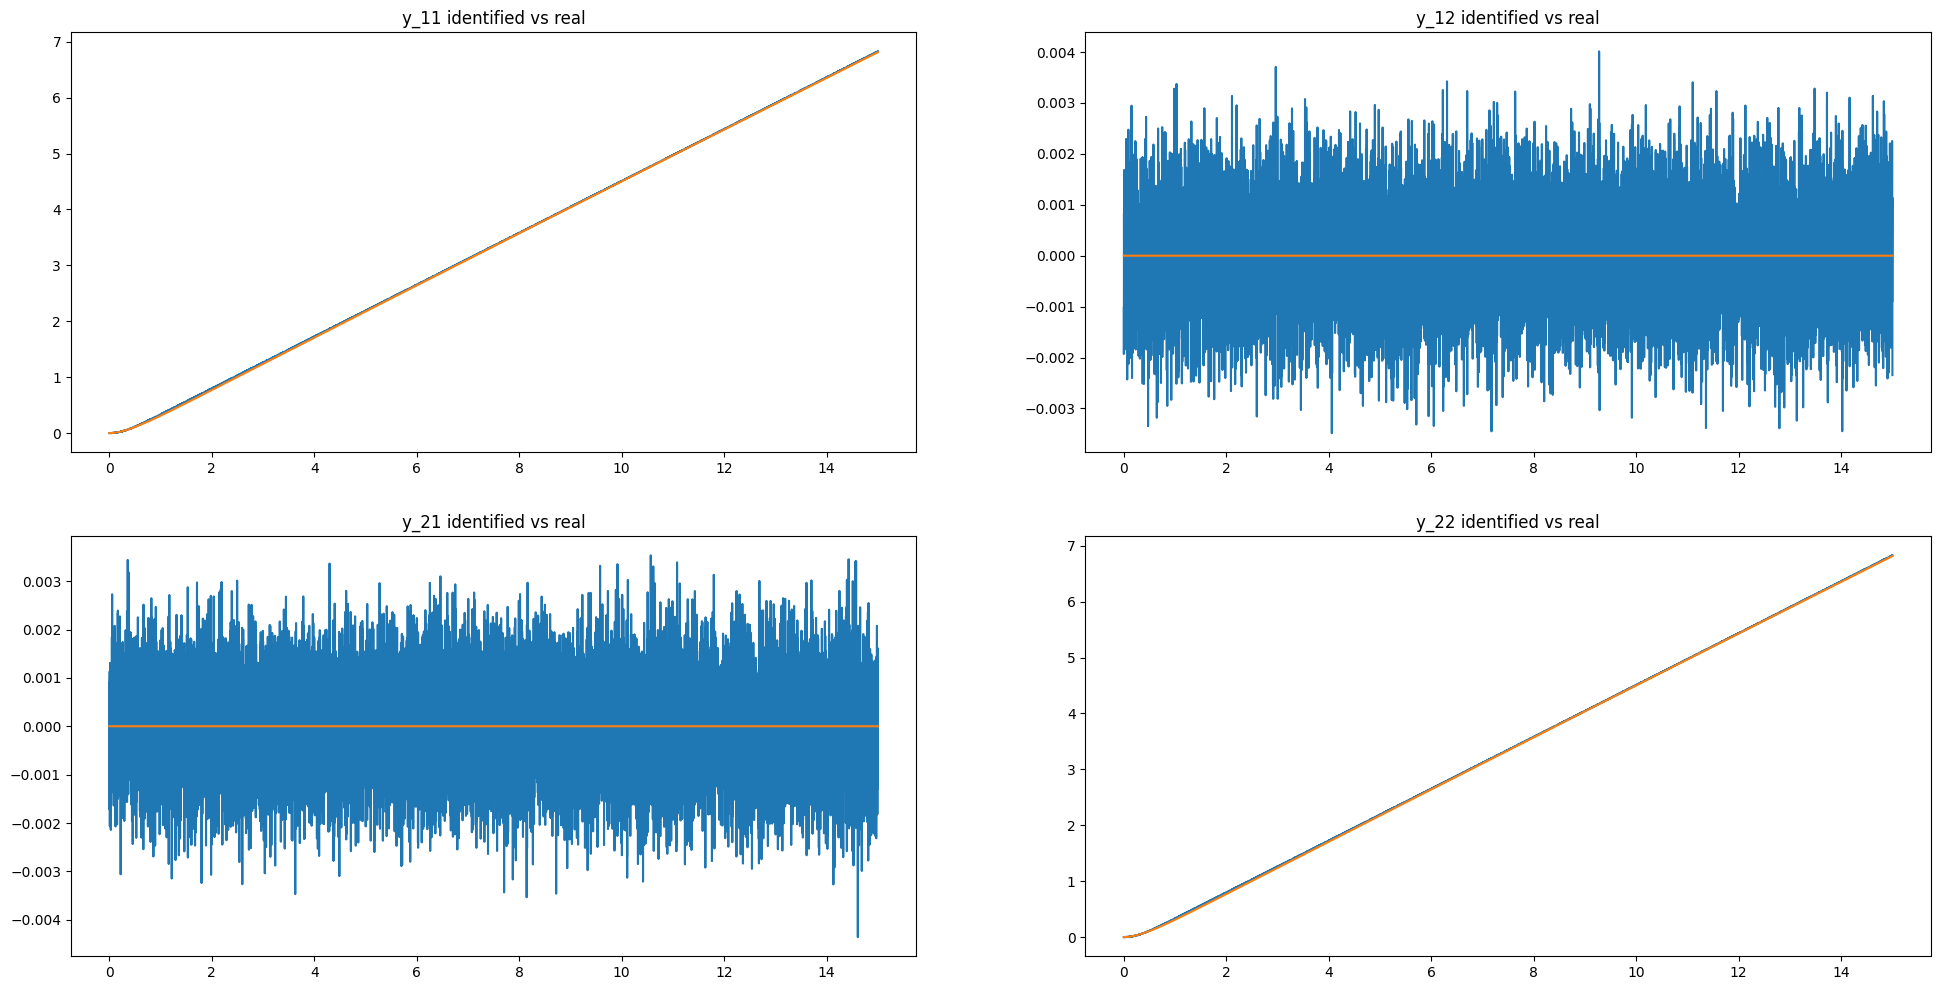
\includegraphics[width=450pt]{p2_4.png}

\textbf{Item 7}

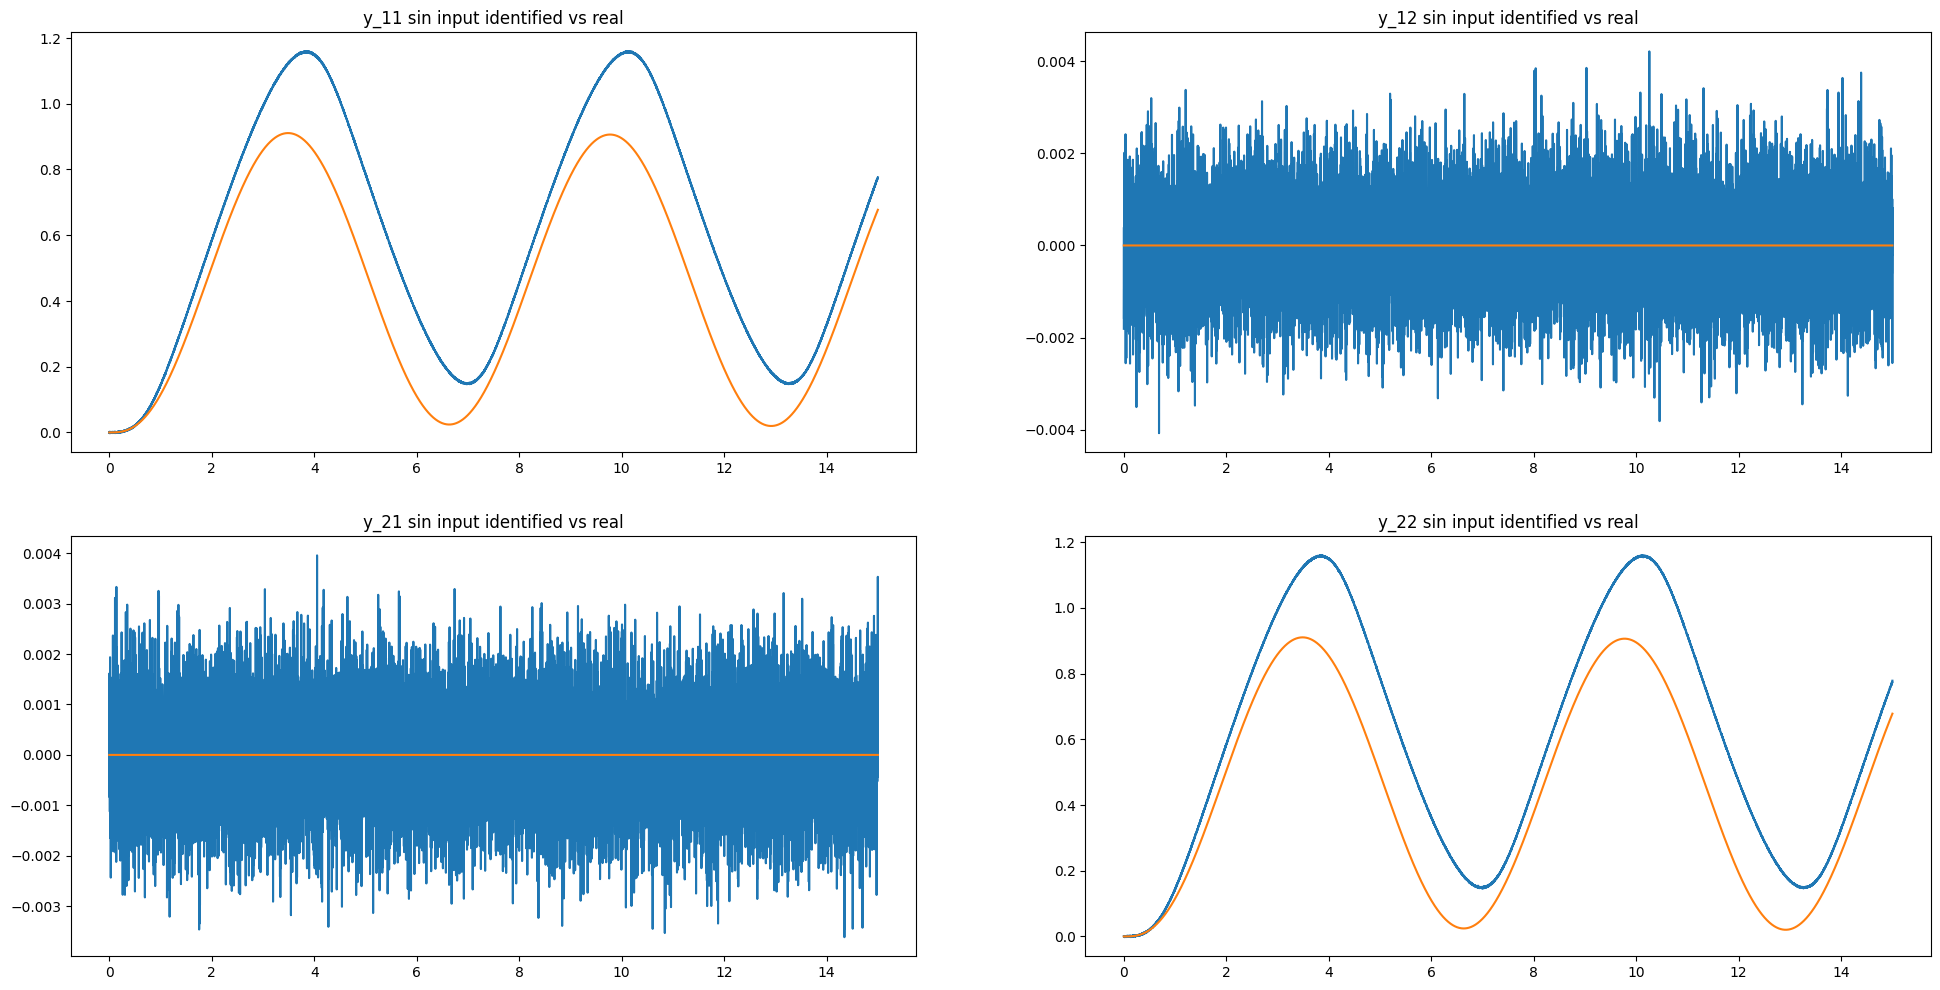
\includegraphics[width=450pt]{p2_5.png}

\end{document}
